\subsection{Tous ensemble}

Toutes les équipes dans l'entreprise travaillent dans un rythme Agile, et chaque équipe choisi l'implémentation qui le convient le plus.

D'un façon global, Bonitasoft travail avec le framework représenté dans la Figure \ref{frame_safe}

\begin{figure}[!ht]
\centering
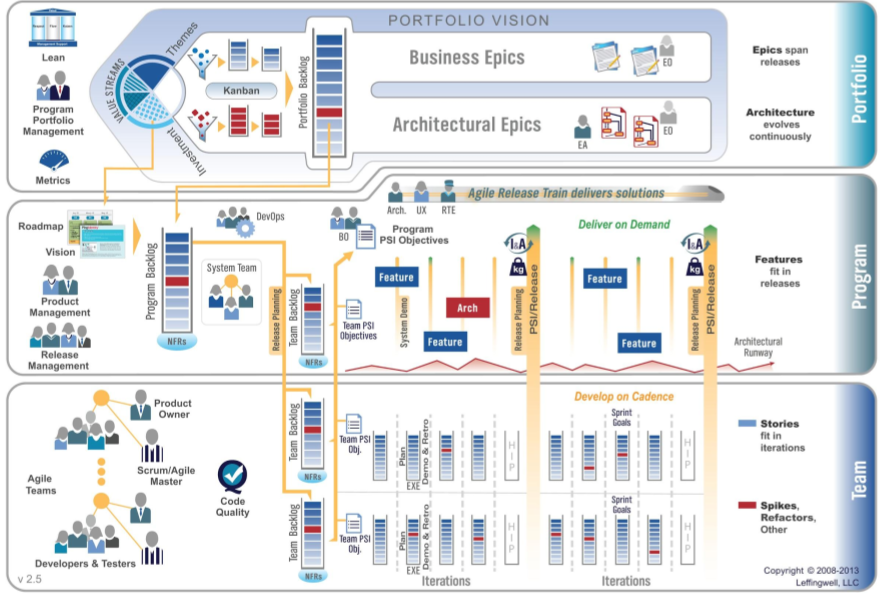
\includegraphics[width=\textwidth,keepaspectratio]{safe_framework.png}
\caption{Cadre de Travail \cite{safe}}
\label{frame_safe}
\end{figure}

Nous voyons dans la partie supérieur que la vision et les fonctionnalités et l'architecture de haut niveau sont définis dans le Comité Produit et le CEO.
Au milieu, le portfolio est traité et organisé par le Product Manager et à la fin il est développé et par l'équipe de développeur avec un Product Owner et le Scrum Master qui dirigent et QA qui assure la qualité du code.

Dans la Figure \ref{fig:example_epic}, nous voyons un exemple des "Epics" avec les "Issues" liés.
\begin{figure}[!ht]
\centering
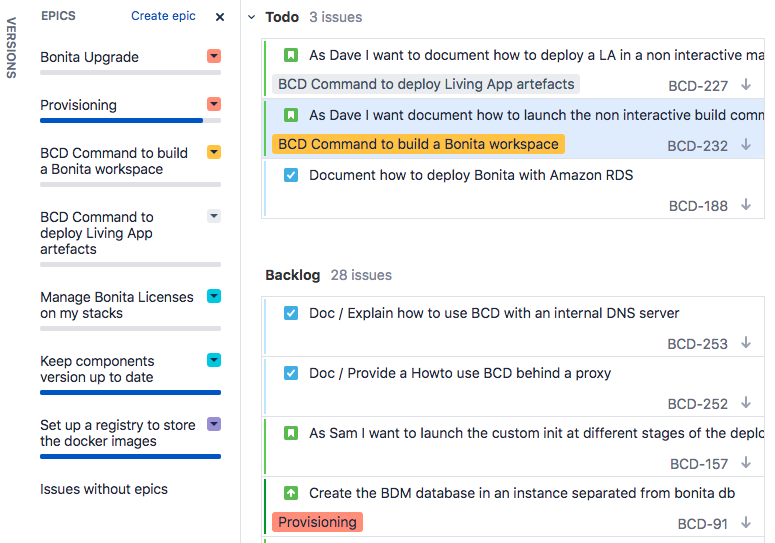
\includegraphics[width=\textwidth,keepaspectratio]{jira_epics_bl.png}
\caption{Exemple de Epics JIRA BCD}
\label{fig:example_epic}
\end{figure}
